\section{Abstract}
Das Teamprojekt DeepRain bestehend aus fünf Studierenden der Masterstudiengänge MSI und BIT startete im Wintersemester 18/19 an der HTWG Konstanz. Das Ziel Projekts ist, innerhalb eines Jahres einen lauffähigen Algorithmus auf Github (thgnaedi/DeepRain) zur Verfügung zu stellen. Dieser soll mit Hilfe von Deep Learning in der Lage sein das Wetter, bzw. den Niederschlag, in Konstanz über den Zeitraum von einer Stunde vorherzusagen. Das einjährige Projekt wird von Prof. Oliver Duerr betreut. 
Eine möglichst genaue Wettervorhersage hat viele offensichtliche Vorteile. Beginnend mit dem täglichen Verlassen des Hauses und der Entscheidung; mit oder ohne den Regenschirm? Vermutlich treffen die meisten diese Entscheidung basierend auf der Wettervorhersage und vertrauen darauf, dass diese auch korrekt ist.
Vorhersagen mit Deep Learning-Unterstützung finden auch eine sehr wichtige Verwendung in der Katastrophenvorhersage und dem Katastrophenmanagement (vgl. \cite[S. 763]{Hanif.2019}). Eine weitere wichtige Rolle spielt es bei der Energieversorgung, beispielsweise bei der Planung der Auslastung von Solar-Panels (vgl. \cite[S. 2]{AndreGensleret.al..}). Die eigentliche Wettervorhersage wird jedoch bisher noch nicht mit Deep Learning-Techniken generiert, dies ist erst ab diesem Jahr bei einigen Anbietern angedacht (vgl. \cite{ChristophFrohlich.2019}. 
\begin{figure}[ht]
\centering
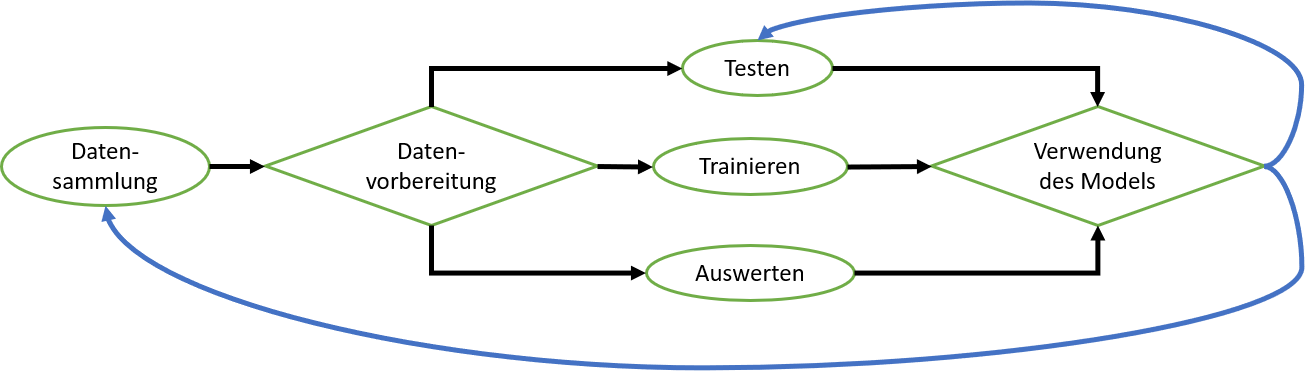
\includegraphics[width=\linewidth]{pics/Deep_learning_prozess}
\caption{Wichtige Schritte im Prozess des DeepRain-Projekts, eigene Darstellung}
\label{fig:deepLearningProcess}
\end{figure}
Im Rahmen des Teamprojekts stand zu Beginn ein einarbeiten in die Prozesse des Maschine-Learnings an, sowie den Stand der Technik zu recherchieren. Daraufhin stand die Datenbeschaffung im Vordergrund und die Qualitätsbewertung der vorhandenen Daten. Im späteren Verlauf des Projekts ging es dann an die Entwicklung des Algorithmus. Der Ablauf dieser Arbeit lehnt sich an diesen, auch in Abbildung~\ref{fig:deepLearningProcess} dargestellten, Prozess an. 

\subsection{Deep Learning}
Deep Learning basiert auf der Optimierung von künstlichen neuronalen Netzen (KNN) und ist eine Weiterentwicklung des Maschine Learning (vgl. \cite[S. 1]{Georgevici.2019}). Ziel von neuronalen Netzen ist es, eine ähnliche Lösungsweise zu ermöglichen, wie im menschlichen Gehirn. Kern ist hier das “Lernen” und das Lösen von Problemen. Neuronale Netze haben sich vor allem wegen ihrer Fähigkeit der Verarbeitung von ständig wachsenden Datenmengen und -komplexität etabliert (vgl. \cite[S. 373]{Welsch.2018}). In einem künstlichen neuronalen Netzwerk müssen im Vorhinein keine Vermutungen über Zusammenhänge festgelegt werden, denn diese werden während des Lernprozesses vom Netz ermittelt (vgl. \cite[S. 581]{Backhaus.2018b}). Ein Neuronales Netz ist 
so aufgebaut, dass es einen bekannten Input gibt, welcher durch einen sogenannten Hidden-Layer läuft. Der Hidden-Layer besteht aus Neuronen in denen das Lernen stattfindet und schließlich ein Output generiert wird. Dabei können einige Variablen, die den Output beeinflussen, festgelegt werden. 
Die Neuronen modifizieren dabei die Daten und leiten diese anschließend weiter (vgl. \cite[S. 373]{Welsch.2018}). Es kann sich auch zwischen einer biologischen oder einer technischen Simulation von Neuronen entschieden werden (vgl. \cite{https:www.facebook.comspektrumverlag.04.12.2014}). Die technische Simulation wird zur Datenverarbeitung und Mustererkennung meist bevorzugt (vgl. \cite{https:www.facebook.comspektrumverlag.04.12.2014}). Dieser Zusammenhang wird in Abbildung~\ref{fig:NeuralVsDeepNeural} dargestellt. 
In dieser Abbildung wird auch ersichtlich, wodurch sich ein tiefes neuronales Netzwerk von einem neuralen Netz unterscheidet. Hier wird gleich mit mehreren Hidden-Layers, die hintereinander liegen, gearbeitet. Die Verwendung mehrerer Hidden-Layers führt dabei laut (\cite[S. 581]{Backhaus.2018b}) zu erfahrungsgemäß korrekteren Lernergebnissen. Das „Lernen“ hängt dann vom Grad der Aktivierung der einzelnen Neuronen ab. Dieser wird durch die bisherigen Ergebnisse durch eine ermittelte Gewichtung einzelner Neuronen bestimmt. Diese Gewichtung wird im Verlauf des Lernens im Netz im besten Fall immer weiter optimiert (vgl. \cite[S. 586]{Backhaus.2018b}).
\begin{figure}[ht]
\centering
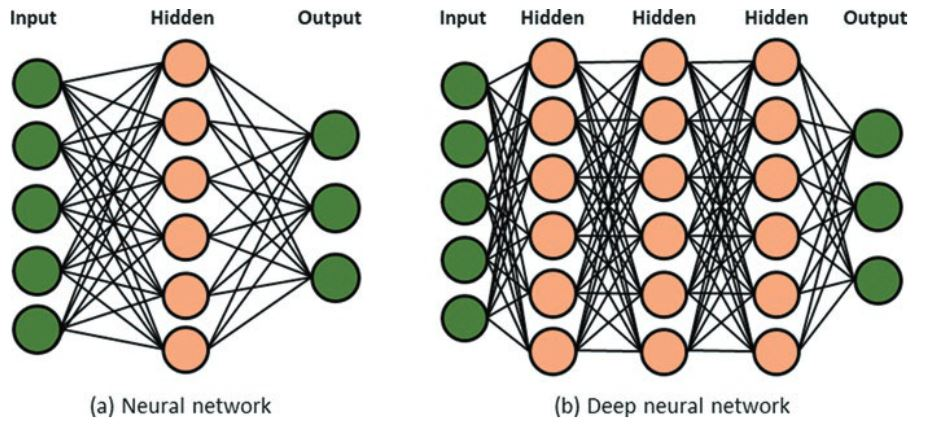
\includegraphics[width=\linewidth]{pics/ANN_for_deep_learning_P35}
\caption{Unterscheidung Neurales Netzwerk und einem mehrstufigen neuronalem Netzwerk, Quelle: ANN for deep learning (Akerkar 2019, S. 35)}
\label{fig:NeuralVsDeepNeural}
\end{figure}
In unserem Projekt soll mithilfe von neuronalen Netzen, das Lernen aus bisherigen Wetterdaten ermöglicht werden, sodass eine möglichst korrekte Wettervorhersage der kommenden Stunde generiert wird.

\subsection{State-of-the-art Wettervorhersage mit Deep Learning}
Obwohl für Deep Learning, Machine-Learning, sowie Neuro- und Lingual-Programming einiges an Literatur zu finden ist, steht die Nutzung zur Wettervorhersage noch am Anfang (vgl. \cite{ChristophFrohlich.2019}). So gibt es auf der Plattform GitHub zum aktuellen Stand (August 2019) gerade einmal eine Handvoll Repositories zum Thema Wettervorhersage mit Deep Learning. Verfahren werden verbessert, die Lernverfahren den Menschlichen Lernen immer ähnlicher, die Entwicklung ist stetig steigend und wie bereits erwähnt sind noch viele Bereiche wie u.a. die Wettervorhersage  ergründbar (\cite[S. 103]{Wick.2017}). Im Bereich der Wettervorhersage bietet sich, in Anlehnung an Abbildung 3, in den meisten Fällen das Supervised Learning an, da eine möglichst genaue Vorhersage erreicht werden soll. Aber auch das  nicht-überwachte Lernen kann interessante Schlüsse zulassen, um eventuell unbekannte Muster zu finden (vgl. \cite[S. 371]{Welsch.2018}). 
